\chapter{Virasoro 代数的张量网络实现}

\section{二维共形场论回顾}

\emph{共形场论} (conformal field theory, CFT)\cite{belavin1984infinite,ginsparg1988applied,francesco2012conformal} 的诞生源于对相变与临界现象的研究。在(二阶)相变点附近,系统应当具有\emph{标度不变性} (scaling invariance);而在二维情况下,标度不变性与共形不变性是等价的。这就意味着可以用满足\emph{共形对称性} (conformal symmetry) 的量子场论——即共形场论——来处理临界系统。

\subsection{共形对称性与能动量张量}

二维 CFT 可以用复平面上的坐标 $z$ 和 $\bar{z}$ 来描述。根据 Cauchy--Riemann 条件,共形变换 $z\to w(z)$ 和 $\bar{z}\to\bar{w}(\bar{z})$ 分别是\emph{全纯} (holomorphic) 和\emph{反全纯} (anti-holomorphic) 的,即它们只是 $z$ 和 $\bar{z}$ 的函数。在这一共形变换下,满足
\begin{equation}
  \phi(z,\bar{z}) \to \phi'(w,\bar{w}) =
  \left( \dv{w}{z} \right)^{-h} \left( \dv{\bar{w}}{\bar{z}} \right)^{-\bar{h}} \phi(z,\bar{z})
  \label{eq:quasi-primary-field}
\end{equation}
变换关系的场 $\phi$ 称为\emph{准初级场} (quasi-primary field),其中
\begin{equation}
  h = \frac12 \bigl( \Delta+s \bigr), \quad \bar{h} = \frac12 \bigl( \Delta-s \bigr)
\end{equation}
称为\emph{共形维数} (conformal dimension),而 $\Delta$ 和 $s$ 分别称为\emph{标度维数} (scaling dimension) 和\emph{自旋} (spin),它们反映了 $\phi$ 在标度和旋转变换下的性质。如果对任意的局部共形变换,式~\eqref{eq:quasi-primary-field} 都成立,则称 $\phi$ 为\emph{初级场} (primary field)。

根据 Noether 定理,(连续)对称性会与某种守恒流相对应。因而我们可以为一个一般的局部坐标变换定义\emph{能动量张量} (energy-momentum tensor),也称\emph{应力张量} (stress tensor)。在共形对称性的条件下,能动量张量 $T^{\mu\nu}$ 可以取为对称且无迹的,即只保留 $T(z)\coloneq T_{zz}(z)$ 和 $\bar{T}(\bar{z})\coloneq T_{\bar{z}\bar{z}}(\bar{z})$,同时它们也是(反)全纯函数\cite{ginsparg1988applied,cardy2010conformal,francesco2012conformal}。$T$ 和 $\bar{T}$ 的共形维数分别为 $(h_T,\bar{h}_T)=(2,0)$ 和 $(h_{\bar{T}},\bar{h}_{\bar{T}})=(0,2)$,即
\begin{equation}
  \Delta_T = \Delta_{\bar{T}} = 2, \quad s_T = 2, \quad s_{\bar{T}} = -2.
\end{equation}

对于共形维数为 $(h,\bar{h})$ 初级场 $\phi$,能动量张量与它的\emph{算子积展开} (operator product expansion, OPE) 具有如下形式:
\begin{equation}
  \begin{aligned}
    T(z) \phi(w,\bar{z}) &\sim
      \frac{h}{(z-w)^2} \phi(w,\bar{z}) + \frac{1}{z-w} \partial_w\phi(w,\bar{z}), \\
    \bar{T}(\bar{z}) \phi(w,\bar{z}) &\sim
      \frac{\bar{h}}{(\bar{z}-\bar{w})^2} \phi(w,\bar{z}) + \frac{1}{\bar{z}-\bar{w}} \partial_{\bar{w}}\phi(w,\bar{z}).
  \end{aligned}
  \label{eq:t-phi-ope}
\end{equation}
而能动量张量与自身的 OPE 则可写为
\begin{equation}
  \begin{aligned}
    T(z) T(w) &\sim
      \frac{c/2}{(z-w)^4} + \frac{2}{(z-w)^2} T(w) + \frac{1}{z-w} \partial_w T(w), \\
    \bar{T}(\bar{z}) \bar{T}(\bar{w}) &\sim
        \frac{\bar{c}/2}{(\bar{z}-\bar{w})^4}
      + \frac{2}{(\bar{z}-\bar{w})^2} \bar{T}(\bar{w})
      + \frac{1}{\bar{z}-\bar{w}} \partial_{\bar{w}}\bar{T}(\bar{w}).
  \end{aligned}
\end{equation}
其中 $(c,\bar{c})$ 称为\emph{中心荷} (central charge)。

\subsection{Virasoro 代数}

二维 CFT 可以进行\emph{径向量子化} (radial quantization),即通过
\begin{equation}
  z = \exp\left( \frac{2\pi\xi}{l} \right), \quad \xi = t+\ii x
  \label{eq:radial-quantization}
\end{equation}
将圆柱面映射到平面上,这样时间 $t$、空间 $x$ 的平移变换就相当于复平面上的缩放与旋转变换。由于等时面 $t\to-\infty$ 被映射到了复平面的坐标原点 $z=\bar{z}=0$,因而可有\emph{态—算符对应} (state-operator correspondence):
\begin{equation}
  \ket{\phi} = \lim_{t\to-\infty}\phi(x,t) \ket{0} = \lim_{z,\bar{z}\to 0} \phi(z,\bar{z}) \ket{0},
\end{equation}
这意味着每一个场算符都可以生成一个对应的量子态(波函数)。

把能动量张量进行模展开,可以得到
\begin{equation}
  \begin{aligned}
    T(z)             &= \sum_{n\in\mathbb{Z}} z^{-n-2} L_n, &\quad
    L_n              &= \frac{1}{2\pi\ii} \oint z^{n+1} T(z) \, \dd z; \\
    \bar{T}(\bar{z}) &= \sum_{n\in\mathbb{Z}} \bar{z}^{-n-2} \bar{L}_n, &\quad
    \bar{L}_n        &= \frac{1}{2\pi\ii} \oint \bar{z}^{n+1} \bar{T}(\bar{z}) \, \dd\bar{z}.
  \end{aligned}
  \label{eq:virasoro-operators}
\end{equation}
式中 $L_n$ 和 $\bar{L}_n$ 称为 \emph{Virasoro 算符} (Virasoro operators),它们构成了 \emph{Virasoro 代数} (Virasoro algebra):
\begin{equation}
  \begin{aligned}
    \bigl[ L_n, L_m \bigr]
      &= (n-m) L_{n+m} + \frac{c}{12} n \bigl( n^2-1 \bigr) \delta_{n+m,0}, \\
    \bigl[ \bar{L}_n, \bar{L}_m \bigr]
      &= (n-m) \bar{L}_{n+m} + \frac{\bar{c}}{12} n \bigl( n^2-1 \bigr) \delta_{n+m,0}, \\
    \bigl[ L_n, \bar{L}_m \bigr] &= 0.
  \end{aligned}
  \label{eq:virasoro-algebra}
\end{equation}
真空态 $\ket{0}$ 需要在全局共形变换下保持不变,这要求
\begin{equation}
  L_n \ket{0} = \bar{L}_n \ket{0} = 0, \quad n \geqslant -1.
\end{equation}
设初级场 $\phi$ 对应的态为 $\ket*{h,\bar{h}}\coloneq\phi(0,0)\ket{0}$。根据式~\eqref{eq:t-phi-ope},可知
\begin{equation}
  L_0       \ket*{h,\bar{h}} = h       \ket*{h,\bar{h}}, \quad
  \bar{L}_0 \ket*{h,\bar{h}} = \bar{h} \ket*{h,\bar{h}}, \quad
  L_n \ket*{h,\bar{h}} = \bar{L}_n \ket*{h,\bar{h}} = 0 \enspace (n > 0).
\end{equation}
代入式~\eqref{eq:virasoro-algebra} 中的对易关系,有
\begin{equation}
  \bigl[ L_0, L_{-n} \bigr] = n L_{-n}, \quad
  \bigl[ \bar{L}_0, \bar{L}_{-n} \bigr] = n \bar{L}_{-n}.
\end{equation}
可以看出 $L_{-n}\ket{0}$ 和 $\bar{L}_{-n}\ket{0}$ 分别是 $L_0$ 和 $\bar{L}_0$ 本征值为 $n$ 的本征态,因而 $L_{-n}$、$\bar{L}_{-n}$ 即可作为升算符,使得共形维数 $h$、$\bar{h}$ 增加 $n$。产生的这些态称为 $\ket*{h,\bar{h}}$ 的\emph{后代} (descendant),它们也可以通过对 $\phi$ 求导得到。

\subsection{环面配分函数}

将圆柱面的 $t\to\pm\infty$ 等时面“粘”在一起便可得到环面。环面的几何由参数 $\tau=\tau_1+\ii\tau_2$ 表示,它需要在变换
\begin{equation}
  \tau \to \frac{a\tau+b}{c\tau+d}, \quad \begin{pmatrix} a & b \\ c & d \end{pmatrix} \in PSL(2,\mathbb{Z})
\end{equation}
下保持不变,其中 $PSL(2,\mathbb{Z})=SL(2,\mathbb{Z})/\mathbb{Z}_2$ 称为\emph{模群} (modular group)。此时配分函数可以写为\cite{cardy1986operator,francesco2012conformal}
\begin{align}
  Z &= \tr \Bigl[ \exp \bigl( -2\pi\tau_2 H \bigr) \exp \bigl( 2\pi\ii\tau_1 P \bigr) \Bigr] \notag \\
    &= \tr \Bigl[
         \exp \Bigl( -2\pi   \tau_2 \Bigl( L_0 + \bar{L}_0 - \frac{c}{12} \Bigr) \Bigr)
         \exp \Bigl(  2\pi\ii\tau_1 \bigl( L_0 - \bar{L}_0 \bigr) \Bigr)
       \Bigr].
\end{align}
其中 $H$ 和 $P$ 分别是 Hamilton 算符和动量算符:
\begin{equation}
% TODO: why c/12; how about c-bar
  H = L_0 + \bar{L}_0 - \frac{c}{12}, \quad P = \ii \bigl( L_0 - \bar{L}_0 \bigr),
\end{equation}
而 $c$ 是中心荷。设场 $\phi_\alpha$ 的共形维数为 $(h_\alpha,\bar{h}_\alpha)$,由 Virasoro 代数可知
\begin{align}
  Z &= \sum_\alpha \exp \Bigl[
         - 2\pi   \tau_2 \Bigl( h_0 + \bar{h}_0 - \frac{c}{12} \Bigr)
         + 2\pi\ii\tau_1 \bigl( h_0 - \bar{h}_0 \bigr)
       \Bigr] \notag \\
    &= \sum_\alpha \exp \Bigl[
         - 2\pi   \tau_2 \Bigl(\Delta_\alpha - \frac{c}{12} \Bigr)
         + 2\pi\ii\tau_1 s_\alpha
       \Bigr],
  \label{eq:torus-partition-function}
\end{align}
其中 $\Delta_\alpha$ 和 $s_\alpha$ 分别是场 $\phi_\alpha$ 的标度维数和自旋。

\subsection{格点近似}
\label{subsec:lattice-approximation}

% TODO:
% 临界格点模型的配分函数可以通过张量网络来描述。以只包含最邻近相互作用的模型为例,其配分函数为
% \begin{equation}
%   Z = \sum_{\sigma_i} \prod_{\langle i,j \rangle} \ee^{-\beta E_{ij}}.
% \end{equation}
% 考虑一个方块附近的四个自由度 $\sigma_i$、$\sigma_j$、$\sigma_k$、$\sigma_l$,令
% \begin{equation}
%   A_{ijkl} = \ee^{-\beta (H_{ij}+H_{jk}+H_{kl}+H_{li})},
% \end{equation}
% 则 $Z$ 可以写成
% \begin{equation}
%   Z = ...
% \end{equation}
% 四个指标的张量 $A_{ijkl}$ 可以排列成一个 $m\times n$ 的网格

% 由于在二维 CFT 中存在态—算符对应,不妨先假想一个以原点为圆心的圆盘,当我们在原点插入一个算符时,圆盘边界处便会产生一个量子态。如果插入的算符是初级场或其后代,那么对应的量子态将会是缩放算符 (dilation operator) 的本征态。利用式~\eqref{eq:radial-quantization} 的逆映射
% \begin{equation}
%   \xi = \frac{l}{2\pi} \log z
% \end{equation}
% 可将复平面变为圆柱,而此时的缩放算符即为沿圆柱轴向的路径积分。

如图~\ref{fig:partition-function-tensor-network} 所示,临界格点模型的配分函数 $Z$ 可以通过张量网络来描述:
\begin{equation}
  Z = \sum_{i_n,j_n,k_n,l_n} \prod_{\alpha=1}^n A_{i_\alpha j_\alpha k_\alpha l_\alpha},
  \label{eq:partition-function-tensor-network}
\end{equation}
其中 $A_{ijkl}$ 是四个指标的张量单元。如果把这个网格的两边“粘”起来,并且只取其中一层,就得到了相应的转移矩阵。同时可以发现,如果在平面的张量网络中插入一个算符,围绕算符边界的张量可以连成一个环,而这个环和圆柱上的转移矩阵(在极限意义下)是等价的。这实际上正是式~\eqref{eq:radial-quantization} 用张量网络语言的表述。因此,转移矩阵的本征态便可用来近似描述在平面上插入的算符。

\begin{figure}[htb]
  % TODO: update image
  \centering
  \includegraphics[width=0.6\textwidth]{images/temp/virasoro-transfer-matrix.pdf}
  \caption[格点模型配分函数的张量网络描述]{格点模型配分函数的张量网络描述。}
  \label{fig:partition-function-tensor-network}
\end{figure}

下面我们来计算转移矩阵的本征值。考虑一个 $m\times n$ 网格上的临界格点模型,并且模型满足周期性边界条件。它的连续极限可以用一个环面上的 CFT 来描述,环面参数为 $\tau=\ii m/n$。根据式~\eqref{eq:torus-partition-function},配分函数为\cite{hauru2016topological}
\begin{equation}
  Z = \sum_\alpha \exp \Bigl[
        - 2\pi \frac mn \Bigl(\Delta_\alpha - \frac{c}{12} \Bigr)
        + mnf + \mathcal{O} \Bigl( \frac{m}{n^\gamma} \Bigr)
      \Bigr],
\end{equation}
其中 $f$ 是热力学极限下每一格点的自由能,而 $\mathcal{O}(m/n^\gamma)$ 则是有限尺寸效应带来的修正。配分函数的“一层”也就是转移矩阵:
\begin{equation}
  Z = \tr M^m,
\end{equation}
因此 $M$ 的本征值为
\begin{equation}
  \lambda_\alpha = \exp \Bigl[
        - \frac{2\pi}{n} \Bigl(\Delta_\alpha - \frac{c}{12} \Bigr)
        + nf + \mathcal{O} \Bigl( \frac{1}{n^\gamma} \Bigr)
      \Bigr].
\end{equation}
由于真空态的标度维数总是 0,我们可以据此消去自由能和有限尺寸修正:
\begin{equation}
  \Delta_\alpha = \frac{n}{2\pi} \bigl( \log\lambda_0 - \log \lambda_\alpha \bigr).
\end{equation}
而如果可以确定能动量张量,还可以利用 $\Delta_T=2$ 的性质来标定 $\Delta_\alpha$:
\begin{equation}
  \Delta_\alpha = \frac{2}{\log\lambda_0 - \log\lambda_T} \bigl( \log\lambda_0 - \log \lambda_\alpha \bigr).
\end{equation}

自旋部分可以通过引入平移算符 $P$ 来得到。在圆柱上,可以写为 $\exp(2\pi\ii P/n)$,而其本征值为 $\exp(2\pi\ii s_\alpha/n)$。在具有平移对称性的模型中,$\exp(2\pi\ii P/n)$ 和转移矩阵 $M$ 对易,因此它们可以被同时对角化。平移算符 $P$ 的张量网络表示如图~\ref{fig:translation-operator} 所示,即把格点平移一个单位。

\begin{figure}[htb]
  % TODO: update image
  \centering
  \[ T_{i_1 i_2 \cdots i_n, \, j_1 j_2 \cdots j_n} = \text{...} \]
  \caption[平移算符 $P$ 的张量网络表示]{平移算符 $P$ 的张量网络表示。}
  \label{fig:translation-operator}
\end{figure}

\section{Virasoro 算符的构造}

类比连续情况下的式~\eqref{eq:virasoro-operators},格点 Virasoro 算符可以表示为
\begin{equation}
  L_n       \sim \sum_{j=1}^N \ee^{ \ii j n \frac{2\pi}{N}} T(j), \quad
  \bar{L}_n \sim \sum_{j=1}^N \ee^{-\ii j n \frac{2\pi}{N}} \bar{T}(j),
  \label{eq:lattice-virasoro-operators}
\end{equation}
其中 $T(j)$ 和 $\bar{T}(j)$ 是能动量张量位于 $j$ 处的格点表示。

对于一些具体的格点模型\cite{koo1994representations,milsted2017extraction},能动量张量 $T$ 可以解析求出。然而在一般情况下,通过配分函数并不能直接得到 $T$ 的表达式。为此,我们需要利用张量网络来构造 Virasoro 算符的近似表示。

如图~\ref{fig:virasoro-construction} 所示,考虑一个以 $A_{ijkl}$ 为单元构成的一般性的张量网络,其中连接维数 $\chi_A=d$。将 $A$ 张量连成一个圆柱得到转移矩阵、与平移算符相连,再对其进行精确对角化,即可按照 \ref{subsec:lattice-approximation} 小节中介绍的方案来确定本征态 $\ket*{\phi_T}$ 或 $\ket*{\phi_{\bar{T}}}$,以及相应的能动量张量 $T$ 或 $\bar{T}$。随后,我们可以把得到的 $T$ 或 $\bar{T}$ 插回由 $A$ 构成的圆柱(即把 $j$ 位置处的 $A$ 张量用 $T$ 或 $\bar{T}$ 取代),再根据式~\eqref{eq:lattice-virasoro-operators} 乘上对应的系数 $\ee^{\pm2\pi\ii j n/N}$,这样就得到了格点上的 Virasoro 算符 $L_n$ 或 $\bar{L}_n$。

\begin{figure}[htb]
  % TODO: update image
  \centering
  \includegraphics[width=0.9\textwidth]{images/temp/virasoro-construction.pdf}
  \caption{在一般的张量网络中确定能动量张量 $T$,并以此来构造 Virasoro 算符。}
  \label{fig:virasoro-construction}
\end{figure}

% TODO: Kac-Moody algebra
当模型具有额外对称性时,相应 CFT 中的 Virasoro 对称性可以推广为 Kac--Moody 对称性。我们可以用完全类似的方法来构造格点 Kac--Moody 算符:
\begin{equation}
  J_n       \sim \sum_{j=1}^N \ee^{ \ii j n \frac{2\pi}{N}} J(j), \quad
  \bar{J}_n \sim \sum_{j=1}^N \ee^{-\ii j n \frac{2\pi}{N}} \bar{J}(j),
\end{equation}
其中 $J(j)$ 和 $\bar{J}(j)$ 是共形维数分别为 $(1,0)$ 和 $(0,1)$ 的流算符。

\subsection{Ising 模型}

二维正方格点上的 Ising 模型,其配分函数为
\begin{equation}
  Z = \sum_{\{\sigma\}} \ee^{-\beta H}
    = \sum_{\{\sigma\}} \ee^{\beta \sum_{\langle ij \rangle} \sigma_i \sigma_j}
    = \sum_{\{\sigma\}} \prod_{\langle ij \rangle} \ee^{\beta \sigma_i \sigma_j}
    = \tr M^m,
\end{equation}
其中 $\sigma\in\{-1,+1\}$ 是 Ising 自旋。它可以按式~\eqref{eq:partition-function-tensor-network} 的形式用张量网络表示,对应的张量单元为
\begin{equation}
  A^{(0)}_{ijkl} = \ee^{-\beta (\sigma_i\sigma_j + \sigma_j\sigma_k + \sigma_k\sigma_l + \sigma_l\sigma_i)}.
\end{equation}
在临界点处,$\beta=\beta_{\text{c}}=\log(1+\sqrt2)/2$。转移矩阵为
\begin{equation}
    M^{i_1 i_2 \cdots i_n}_{k_1 k_2 \cdots k_n}
  = \sum_{j_1, j_2, \ldots, j_n} \prod_{\alpha=1}^n A^{(0)}_{i_\alpha j_\alpha k_\alpha j_{\alpha+1}}
  = \text{[[TODO:]]}
  % = \DiagramI.
\end{equation}

在实际计算中,可以对张量 $A$ 进行粗粒近似以提高精度,如图~\ref{fig:virasoro-blocking} 所示。例如可将 4 个 $A$($\eqcolon A^{(0)}$)组合成一个更大的 $A^{(1)}$,也可不断重复使得 $A^{(i)}$ 逐渐接近不动点张量。在这一过程中,连接维数 $\chi_{A^{(i)}}=d^{2^i}$ 会迅速增大,因此往往还需要进行截断。实际上,这也就是利用 TRG\cite{levin2007tensor} 或者 TNR\cite{evenbly2015tensor,evenbly2017algorithms} 等张量网络算法来寻找不动点张量的操作。

\begin{figure}[htb]
  % TODO: update image
  \centering
  \includegraphics[width=0.9\textwidth]{images/temp/virasoro-blocking.pdf}
  \caption{对张量 $A$ 进行粗粒近似。}
  \label{fig:virasoro-blocking}
\end{figure}

在确定能动量张量的过程中,为了使得 $T$ 或 $\bar{T}$ 之后能被插入到圆柱中,它们必须有 4 个指标。如果使用 4 个 $A^{(0)}$ 张量组成转移矩阵,虽然得到的本征态形状满足要求,但此时 $\ket*{\phi_T}$ 和 $\ket*{\phi_{\bar{T}}}$ 将会是简并的(由于 $-2\bmod4=+2$,计算得到的自旋都是 $+2$)。因此我们将使用 $N=8$ 的转移矩阵来进行精确对角化以得到能谱数据(见表~\ref{tab:ising-spectrum}),并从中找到标度维数 $\Delta\approx2$、自旋 $s=\pm2$ 的 $\ket*{\phi_T}$ 和 $\ket*{\phi_{\bar{T}}}$,并将它们从 8 个指标、$\chi=2$ 变形为 4 个指标、$\chi=4$ 的张量 $T$ 和 $\bar{T}$。对于 Ising 模型,此时已经可以得到较好的精度,因此在这一步中我们没有使用粗粒近似后的 $A^{(i)}$ 张量。

\begin{table}[htb]
  \caption{Ising 模型的能谱数据。圆柱(转移矩阵)的尺寸由 4 取到 24,并且外推至无穷大。注意此处 $\Delta_\alpha$ 没有根据 $\Delta_T=2$ 的性质来进行标定。}
  \label{tab:ising-spectrum}
  \newcommand{\header}[2]{%
    \textsubscript{\footnotesize#1}\,\textbackslash\,\textsuperscript{\footnotesize#2}}
  \centering\footnotesize
  \begin{tabular}{*{9}{c}}
    \toprule
      \header{自旋}{尺寸} & 4        & 8        & 12       & 16       & 20       & 24       & $\infty$     & 理论值 \\
    \midrule
      0                   & 0.123499 & 0.124606 & 0.124823 & 0.124900 & 0.124936 & 0.124955 & 0.12522\,(6) & $\frac18$     \\
      0                   & 1.026740 & 1.006488 & 1.002868 & 1.001610 & 1.001030 & 1.000715 & 0.9961\,(11) & 1             \\
      $\pm1$              & 1.245699 & 1.151345 & 1.136446 & 1.131388 & 1.129074 & 1.127824 & 1.107\,(5)   & $1{+}\frac18$ \\
      $\pm1,\pm2$         & 2.569513 & 2.098365 & 2.041544 & 2.022974 & 2.014590 & 2.010090 & 1.916\,(30)  & 2             \\
      0                   & 2.367899 & 2.178085 & 2.148069 & 2.137876 & 2.133212 & 2.130692 & 2.089\,(11)  & $2{+}\frac18$ \\
      $\pm2$              & -        & 2.369005 & 2.223018 & 2.178379 & 2.158670 & 2.148201 & 2.043\,(19)  & $2{+}\frac18$ \\
    \bottomrule
  \end{tabular}
\end{table}

除了直接考察能谱数据,我们还可以通过分析能动量张量的两点关联函数来检验其正确性,它们可以使用 iTEBD 算法来计算(见 [[TODO:]])。首先,我们使用 $A$ 张量来构建一个无限一维链 (iMPS),并将其转化为正则形式。接下来,我们通过对 iMPS 进行虚时演化来计算配分函数。再把 $T$ 插入配分函数中,即可计算得到关联函数,其结果如图~\ref{fig:ising-correlation-functions} 所示。可以发现 $T$ 的两点关联函数存在幂律行为,并且拟合得到的标度维数与表~\ref{tab:ising-spectrum} 中的能谱数据大致相符。

\begin{figure}[ht]
  \centering
  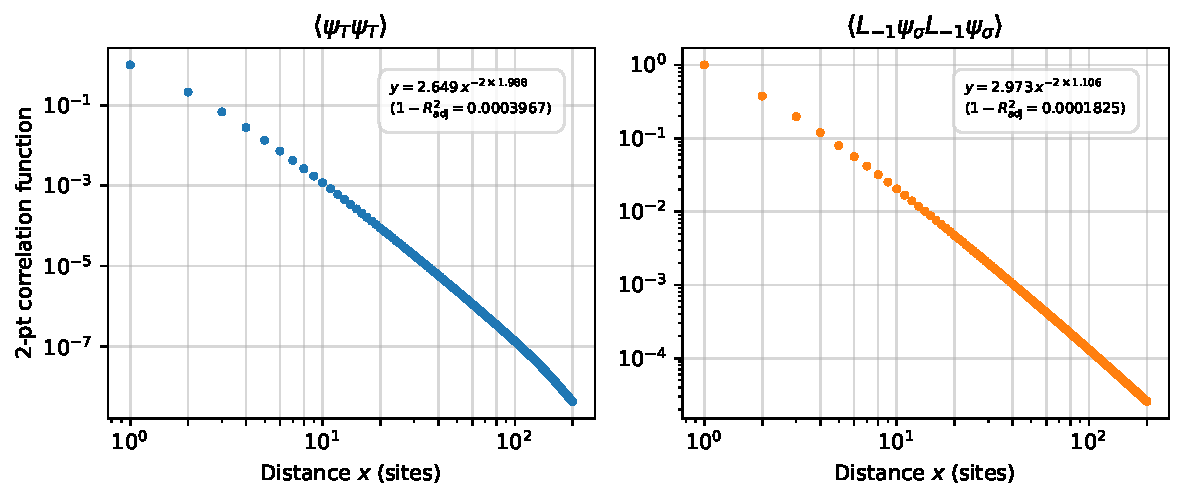
\includegraphics[width=0.9\textwidth]{images/fibonacci/ising-correlation-function.pdf}
  \caption[Ising 模型中能动量张量 $T$ 和 $L_{-1}\psi_\sigma$ 的两点关联函数]{Ising 模型中能动量张量 $T$(左图)和 $L_{-1}\psi_\sigma$(右图)的两点关联函数。为了避免计算本征值时有限尺寸效应导致的误差,以及 iTEBD 算法中的长程累积误差,我们只取 $x=10$ 到 100 区间的数据来拟合幂律公式 $y=Ax^{-2\Delta}$,此时分别得到 $\Delta=1.988$ 和 1.106。它们与 Ising 能谱的理论结果($\Delta=2$ 和 $1+1/8$)基本相符。}
  \label{fig:ising-correlation-functions}
\end{figure}

注意到此时 $T$ 和 $\bar{T}$ 的形状和 $A^{(1)}$ 是相同的,我们便可以按照图~\ref{fig:virasoro-construction} 的方法来构造 Virasoro 算符。这里我们仍然选取 $N=8$ 的圆柱,但组成它的张量单元都是经过粗粒近似的 $A^{(1)}$,其连接维数 $\chi=4$。

\begin{figure}[htb]
  % TODO: update image
  \centering
  \includegraphics[width=0.5\textwidth]{images/temp/virasoro-operator.pdf}
  \caption{Virasoro 算符作用于本征态上。}
  \label{fig:virasoro-operator}
\end{figure}

为了检验这一方法的正确性,我们把得到的 Virasoro 算符 $L_n$ 和 $\bar{L}_n$ 进一步作用在 $N=8$、$\chi=4$ 圆柱的本征态 $\ket*{\phi_\alpha}$ 上(如图~\ref{fig:virasoro-operator} 所示)。在 CFT 中,Virasoro 算符起到升降算符的作用,使得
\begin{equation}
  L_n         \ket{\Delta_\alpha, s_\alpha} \propto \ket{\Delta_\alpha-n, s_\alpha-n}, \quad
  L_{\bar{n}} \ket{\Delta_\alpha, s_\alpha} \propto \ket{\Delta_\alpha-n, s_\alpha+n}.
\end{equation}
因此只需考察矩阵元 $\langle\phi_\beta|L_n|\phi_\alpha\rangle$ 的值,即可判断 $L_n$ 和 $\bar{L}_n$ 是否能将 $\ket*{\phi_\alpha}$ 映射到相应的态上。我们的计算结果显示,在 Ising 模型中,对于 $N=8$、$\chi=4$ 圆柱的本征态,近似有
\begin{equation}
  \frac{\lVert \langle\phi_\beta|L_n|\phi_\alpha\rangle \rVert}{\lVert \ket*{\phi_\beta} \rVert \cdot \lVert L_n\ket*{\phi_\alpha} \rVert} \gtrsim 0.9, \quad
  n=\pm1, \pm2.
\end{equation}
这说明通过本方法计算得到的格点 Virasoro 算符与 CFT 的理论预言基本是一致的,并且具有比较好的精度。在图~\ref{fig:virasoro-ising-spectra} 中,我们给出了这些格点 Virasoro 算符作用的示意图。矩阵元的数据可以在文献 \parencite{wang2022virasoro} 的补充材料中找到。我们观察到,在这些矩阵元中,有一些数据的精度相对较低(与正确值相差 1 到 2 个数量级)。造成这种问题的原因主要是格点模型的有限尺寸效应:一方面,在比较小的圆柱中,CFT 的不同本征态实际上是存在交叠的;另一方面,格点 Virasoro 算符也是通过对有限大小的圆柱进行精确对角化求得的,本身也存在一定误差。

Virasoro 算符的正确性同样可以通过两点关联函数来检验。在图~\ref{fig:ising-correlation-functions} 中,我们考察了 $L_{-1}\psi_\sigma$ 的关联函数,拟合得到的标度维数与理论值($1+1/8$)也是基本一致的。

\begin{figure}[htb]
  \centering
  \includegraphics[width=0.4\textwidth]{images/temp/ising_lm1.pdf}    \quad
  \includegraphics[width=0.4\textwidth]{images/temp/ising_lbarm1.pdf} \\
  \includegraphics[width=0.4\textwidth]{images/temp/ising_l1.pdf}     \quad
  \includegraphics[width=0.4\textwidth]{images/temp/ising_lbar1.pdf}  \\
  \includegraphics[width=0.4\textwidth]{images/temp/ising_lm2.pdf}    \quad
  \includegraphics[width=0.4\textwidth]{images/temp/ising_lbarm2.pdf} \\
  \includegraphics[width=0.4\textwidth]{images/temp/ising_l2.pdf}     \quad
  \includegraphics[width=0.4\textwidth]{images/temp/ising_lbar2.pdf}
  \caption{Virasoro 算符在 Ising 模型的能谱上的作用示意图。}
  \label{fig:virasoro-ising-spectra}
\end{figure}

\subsection{Fibonacci 模型}

在很大程度上,Ising 模型具有一定的特殊性,例如有限尺寸效应影响较小。对于更一般的模型,无论是计算并确定圆柱本征态,还是构造对应的 Virasoro 算符,都比较困难。本小节我们将考察 $\mathbb{Z}_3$ parafermion CFT,它可以通过为 Fibonacci 拓扑序添加适当的边界条件而得到。

\section{能动量张量的确定}
